\documentclass[twocolumn]{article}
\usepackage[utf8]{inputenc} % TODO?
\usepackage{url}
\usepackage{listings}
\lstset{
  basicstyle=\ttfamily\small,
  columns=fixed,
  fontadjust=true,
  basewidth=0.5em
}
\usepackage{alltt}
\usepackage{graphicx}
\usepackage{caption}
\captionsetup[figure]{font=small,labelfont=normalsize,justification=centering}
%\usepackage[showframe]{geometry}
\graphicspath{ {./images/} }

\title{Streaming Merkle Proofs within Binary Numeral Trees}
\author{
Luke Champine\\
The Sia Foundation\\
luke@sia.tech
}

\begin{document}
\frenchspacing

\maketitle


\subsection*{Abstract}
We describe the \textit{binary numeral tree}---a type of binary tree uniquely suited to processing unbounded streams of data---and present a number of algorithms for efficiently constructing and verifying Merkle proofs within such trees. Specifically, we present existence proofs for single leaves, for a contiguous range of leaves, and for multiple disjoint ranges. We also introduce Merkle ``diff'' proofs, which assert that an arbitrary modification was correctly applied to an existing tree. Each algorithm, operating on a tree with $n$ leaves and $k$ disjoint proof ranges, requires $\mathcal{O}(\log_2(n))$ space and $\mathcal{O}(n)$ time, and yields proofs of size $\mathcal{O}(k\log_2 (n))$. Furthermore, each algorithm operates in streaming fashion, requiring only a single in-order pass over the leaf data.


\section{Introduction}

Merkle trees\cite{Merkle} are the prototypical authenticated data structure: they permit the construction and verification of compact cryptographic proofs that assert various properties of the tree, most commonly the presence of a specific leaf within the tree (an \textit{existence proof}). They are frequently employed in protocols that deal with large amounts of data in an untrusted context, such as BitTorrent, Certificate Transparency, and cryptocurrencies. Recent renewed interest in Merkle trees has given rise to an explosion of tree variants, including sparse Merkle trees, bloom trees, and others.

This paper discusses Merkle proofs in the context of a single tree type: the binary numeral tree, or BNT. A BNT consists of a set of perfect binary subtrees of distinct sizes---its \textit{eigentrees}---recursively joined smallest-to-largest into a single tree. For any number of leaves $n$, there is exactly one possible BNT structure, which we will refer to as the $n$-BNT. As such, it may be instructive to conceive of the BNT as a tree structure imposed upon a flat sequence of leaves, rather than as a mutable object into which leaves are progressively inserted.

Binary numeral trees are so named because of their correspondence to the binary numeral system: the eigentrees of an $n$-BNT correspond to the 1 bits in the binary representation of $n$. For example, the 11-BNT in Figure \ref{img-bnt} comprises eigentrees of sizes $2^0$, $2^1$, and $2^3$. Additionally, an $n$-BNT can be transformed into an $(n+1)$-BNT via a process analgous to incrementing a binary integer: to ``add'' a new leaf to the 11-BNT, we begin by merging the new leaf---itself a $2^0$ subtree---with the existing $2^0$ eigentree, forming a $2^1$ subtree; we then ``carry'' this subtree, merging it with the existing $2^1$ eigentree, to form a $2^2$ subtree. Here, the process stops, as there is no other $2^2$ eigentree to merge with. The result is a 12-BNT, comprising a $2^2$ eigentree and a $2^3$ eigentree.

\begin{figure*}[t]
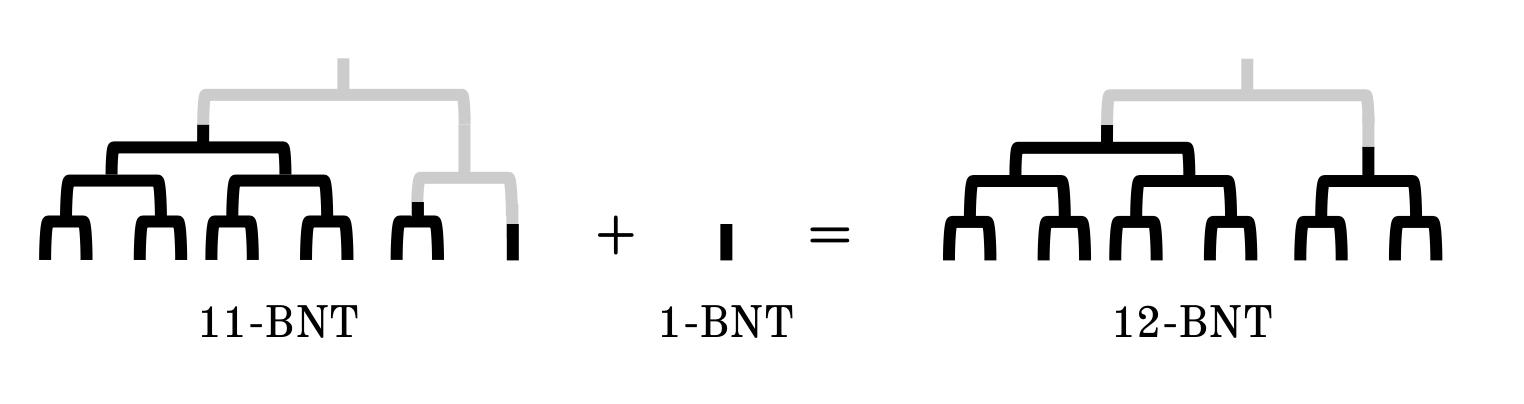
\includegraphics[scale=0.4]{bnt}
\centering
\caption{Adding a leaf to an 11-BNT to produce a 12-BNT. Eigentrees are highlighted in black.}
\label{img-bnt}
\end{figure*}

What makes the BNT structure interesting is that it can ``ingest'' an unbounded number of leaves in this way while preserving two important properties. First, the tree's bottom layer remains flat, with the maximum leaf depth capped at $\left \lceil{\log_2(n)}\right \rceil$. Second, the eigentrees are immutable: adding a new leaf may cause existing eigentrees to be merged, but no eigentree will ever gain or lose leaves.

These properties are particularly desirable in a Merkle tree. The depth limit prevents proofs from growing too large: existence proofs require $\mathcal{O}(\log_2(n))$ space and time, regardless of which leaf is chosen. More importantly, since the eigentrees are immutable, their Merkle root hash will never change; thus, once we have finished processing an eigentree, we can discard its leaves, retaining only the root.

Another convenient property of BNTs is that they inherit an isomorphism from perfect binary trees: the path from any leaf $i$ to the root of the tree is uniquely described by the bit pattern of $i$. As we will demonstrate, this property can be exploited for various purposes. Moreover, since computer hardware is designed for operating on binary integers, the resulting algorithms are extremely efficient in practice.


\section{Related Work}

Given its favorable properties, it should not come as a surprise that the BNT structure has been independently discovered and employed in multiple projects, including Certificate Transparency\cite{RFC6962}, the Sia storage protocol\cite{Sia}, Dryja's Utreexo\cite{Utreexo} proposal for Bitcoin, and the BLAKE3 hash function\cite{BLAKE}, all of which perform Merkle operations on input streams of arbitrary size. Variations on the BNT are also known, including ``history trees''\cite{CrosbyWallach}, ``Merkle Mountain Ranges''\cite{Todd}, and the (unnamed) tree structure used in BitTorrent, all of which preserve the ``flat base'' property of the BNT, but differ in how they handle imperfect tree sizes and/or how they combine eigentree roots.

It is notable that all of the aforementioned examples operate specifically on \textit{Merkle} BNTs. While the BNT structure is not necessarily authenticated, it would appear that no unauthenticated applications have yet been discovered.

Most existing work on Merkle trees is concerned with existence proofs for single leaves within a tree. Ramabaja and Avdullahu\cite{CMM} explore existence proofs for multiple disjoint leaf ranges, but assume random-access input. To our knowledge, this is the first treatment of Merkle trees (of any type) that describes streaming algorithms for constructing and verifying multi-range proofs.

\begin{figure*}[t]
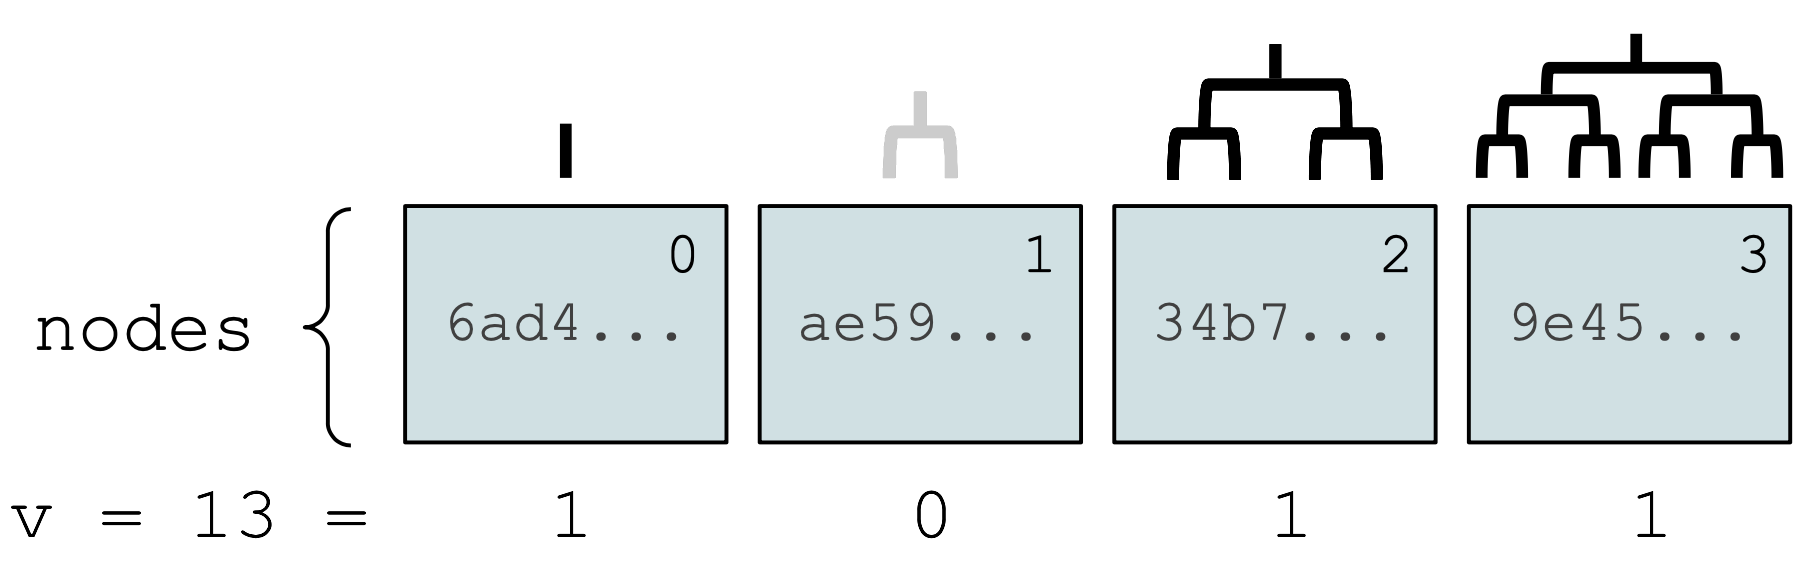
\includegraphics[scale=0.3]{stack}
\centering
\caption{Visualization of the stack structure for a 13-BNT. The hash in position 1 is ignored because its corresponding bit is 0. Note that array is ordered ``little-endian'', matching the endianness of $v$.}
\label{img-stack}
\end{figure*}

% TODO: if array is fixed-size, why not start at end?
% endianness doesn't cause more copying...

\section{Streaming Merkle Roots}

We begin by presenting an algorithm for computing the Merkle root of a BNT from an input stream of unknown size. As a refresher, to compute the root of a perfect tree with $n$ leaves, we could employ the elegant recursive algorithm:

\begin{minipage}[c]{0.95\textwidth}
\begin{lstlisting}
fn PerfectRoot(stream, n):
  if n == 1:
    return leafHash(readLeaf(stream))
  else:
    return parentHash(
      PerfectRoot(stream, n/2),
      PerfectRoot(stream, n/2))
\end{lstlisting}
\end{minipage}

(In the interest of brevity, we will omit the definitions of procedures such as \verb`readLeaf`, \verb`parentHash`, etc. whose meaning is clear from their surrounding context. All such procedures will be written in \verb`camelCase`, while defined procedures will use \verb`PascalCase`.)

This algorithm could also be modified to work on a BNT by splitting the input at $2^{\left \lceil{\log_2(n)}\right \rceil - 1}$ rather than $n/2$. Unfortunately, in a streaming context, we do not know $n$, so a different approach is needed.

In lieu of recursion, our algorithm uses an explicit ``stack'' of accumulated values. We repeatedly read the next leaf from the stream, hash it to create a node of height $2^0$, and add it to our stack with the \verb`Insert` procedure, which merges pairs of nodes with height $2^k$ into nodes of height $2^{k+1}$, ``carrying'' as necessary. Our stack is thus a compressed representation of a BNT, storing only its \textit{eigenroots}---the root hashes of the eigentrees. When the stream is exhausted, we apply a standard right-fold to the eigenroots to obtain the total root of the $n$-BNT.

\begin{minipage}[c]{0.95\textwidth}
\begin{lstlisting}
fn Insert(s, k, node):
  if has(s, k):
    node <- parentHash(node, get(s, k))
    delete(s, k)
    return Insert(s, k+1, node)
  else:
    s <- set(s, k, node)
    return s
    
fn Finalize(s):
  nodes <- []
  for k in len(s)..0:
    if has(s, k):
      nodes <- append(nodes, get(s, k))
  return foldr1(nodes, parentHash)

fn Root(stream):
  stack <- makeStack()
  while !empty(stream):
    node <- leafHash(readLeaf(stream))
    stack <- Insert(stack, 0, node)
  return Finalize(stack)
\end{lstlisting}
\end{minipage}

\pagebreak

This pseudocode implies that \verb`stack` is a map from heights to nodes; in practice, we can implement this data structure using a simple array, \verb`nodes`, and an integer \verb`v`. Each time we read a leaf, we increment \verb`v`; thus, thanks to the BNT isomorphism, the bit pattern of \verb`v` will correspond to the ``live'' indices of \verb`nodes`. That is, if \verb`v = 13`, we will know that \verb`nodes` contains eigenroots at indices 0, 2, and 3, while the other indices should be ignored. Consequently, an explicit \verb`delete` procedure is unnecessary. As an added bonus, the stack may be ``reset'' simply by setting \verb`v = 0`.



\begin{figure*}[t]
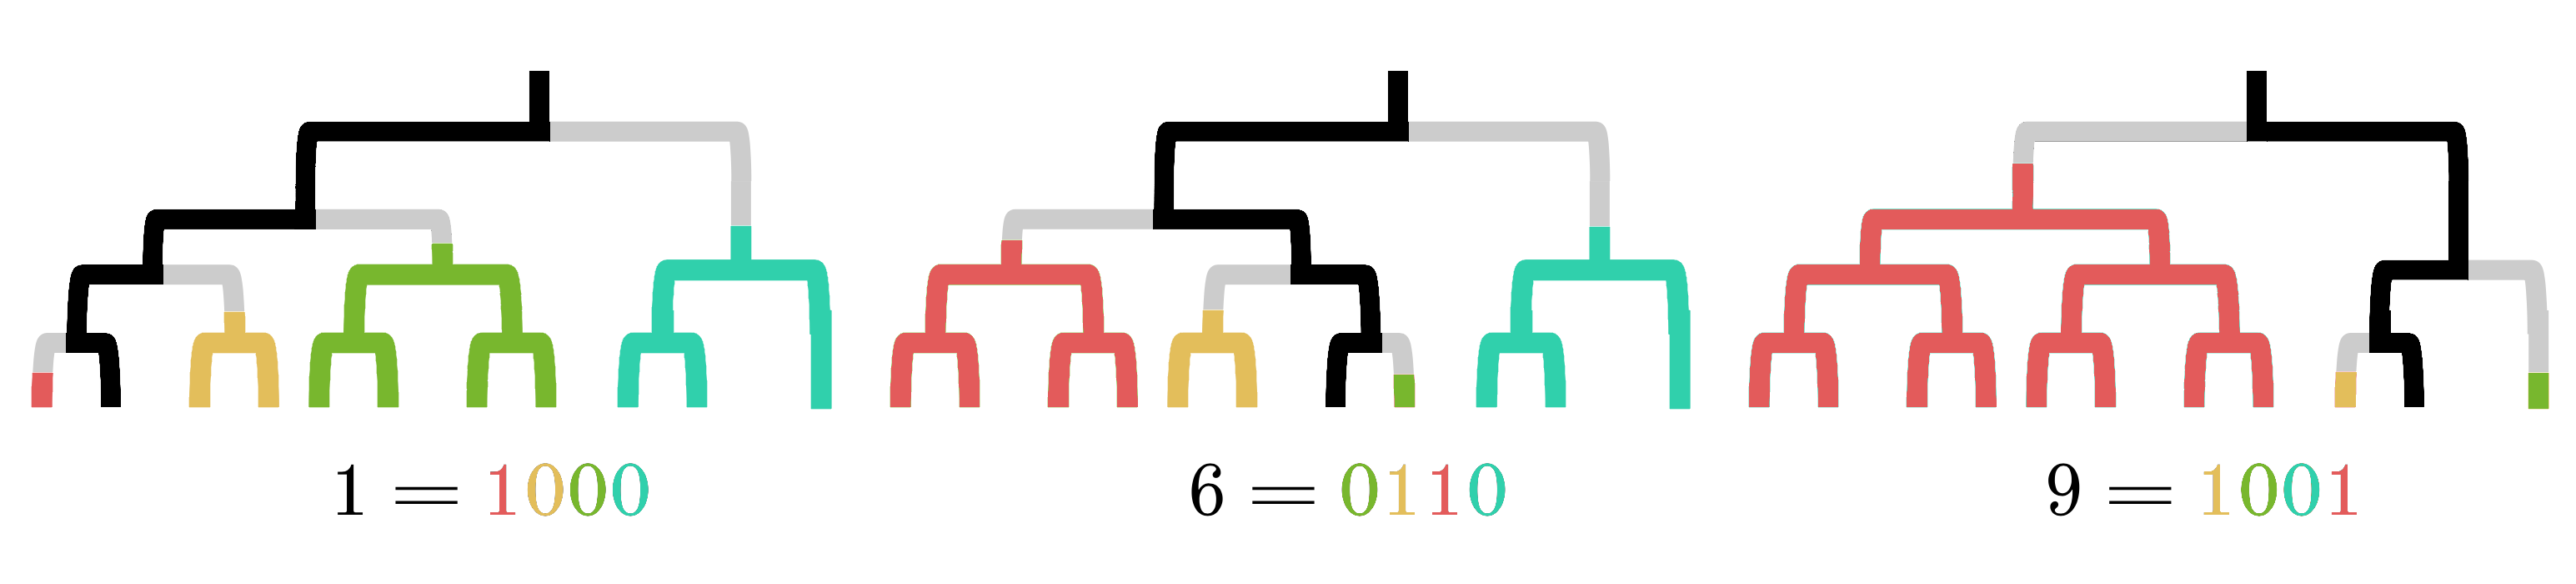
\includegraphics[scale=0.24]{paths}
\centering
\caption{Single-leaf Merkle proofs for leaf indices 1, 6, and 9, demonstrating the correspondence between proof paths (highlighted in black) and index bits. Note the ``missing'' subtree in the path for index 9.}
\label{img-path}
\end{figure*}

\section{Single-leaf Proofs}

A single-leaf proof---the simplest form of Merkle proof---asserts the presence of a single leaf within the tree by presenting the verifier with a set of \textit{sibling hashes}. The verifier combines the leaf and sibling hashes as they would appear within the tree; if the resulting root matches the root previously known to the verifier, then the proof is considered valid.


Merkle proofs conventionally proceed ``vertically,'' from the leaf to the root. This is arguably the most intuitive way to build and verify proofs, and it can directly leverage the aforementioned leaf index isomorphism. That is, to build a proof for leaf $i$, an algorithm can iterate over the bits of $i$, with each bit determining the next subtree to hash; and to verify a proof for leaf $i$, the bits of $i$ can be examined to determine the relative position of each sibling hash in the proof.

This approach can be modified for use in BNTs as well. Unfortunately, while elegant, it is ill-suited to working with streams of unknown size. In a streaming context, we want an algorithm that examines each leaf in order; a leaf-to-root algorithm would entail jumping back and forth in the stream repeatedly.

How might we construct a single-leaf proof in streaming fashion? Looking at the proof for index 6 in Figure \ref{img-path}, this would mean first computing the root of the first 4 leaves (moving left-to-right); then of the next 2 leaves; then skipping over leaf 6 itself; then computing the root of the next leaf, and finally the root of the last 3 leaves.

We know that each of these roots corresponds to a bit in the leaf index. Observe that each subtree root to the left of the leaf corresponds to a \verb`1` bit: there are \verb`1` bits in positions $2^2$ and $2^1$, matching the roots of the first $2^2$ leaves and the following $2^1$ leaves, respectively. Likewise, each root to the right of the leaf corresponds to a \verb`0` bit, with one caveat: the \verb`0` bit at position $2^3$ implies a subtree with 8 leaves, but only three remain in the tree. In this case, the root simply covers fewer leaves than its bit suggests.

Further observe that the ``left subtrees'' shrink in size until reaching the proof index, whereas the ``right subtrees'' grow in size thereafter. So, to construct the proof, we first examine the 1 bits of the index, moving from most-significant to least-significant; for each bit position $k$, we read $2^k$ leaves from the stream and compute their Merkle root, which we append to our proof. We then read a single leaf---the leaf being proven. Finally, we examine the 0 bits, this time moving from least-significant to most-significant, again computing the Merkle root of each sequence of $2^k$ leaves and appending them to our proof. Here, though, we must be careful: there may be fewer than $2^k$ leaves remaining in the stream, as in Figure \ref{img-path}. To account for this, we define a helper procedure, \verb`Subroot`, that returns the root of \textit{at most} $2^k$ leaves.

\begin{figure*}[t]
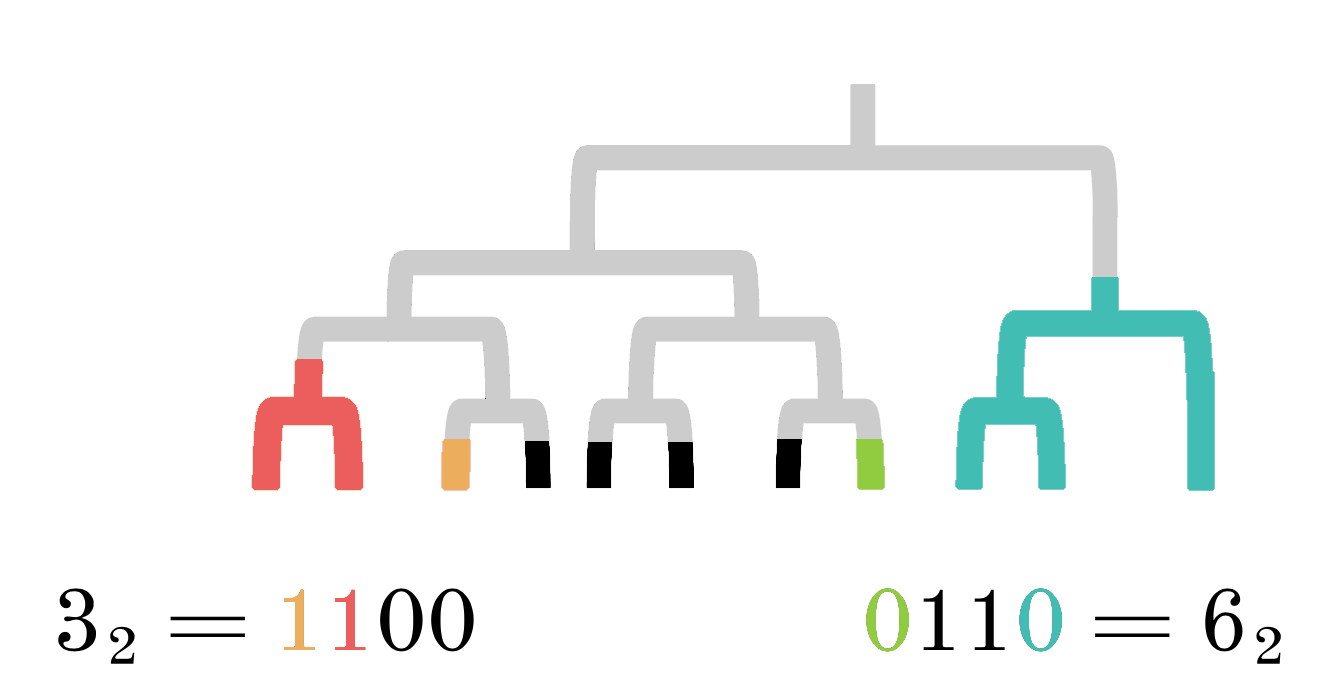
\includegraphics[scale=0.24]{range}
\centering
\caption{Single-range Merkle proof for leaf indices 3, 4, 5, and 6. The \texttt{1} bits of 3 correspond to ``left-hand'' sibling hashes, while the \texttt{0} bits of 6 correspond to ``right-hand'' sibling hashes. The other bits have no significance.}
\label{img-range}
\end{figure*}


\begin{minipage}[c]{0.95\textwidth}
\begin{lstlisting}
fn Subroot(stream, k):
  return Root(limit(stream, 1<<k))
\end{lstlisting}
\end{minipage}

\noindent The proof algorithm is then straightforward:

\begin{minipage}[c]{0.95\textwidth}
\begin{lstlisting}
fn ProveLeaf(stream, index):
  proof <- []
  for k in reverse(ones(index)):
    node <- Subroot(stream, k)
    proof <- append(proof, node)
  leaf <- readLeaf(stream)
  for k in zeros(index):
    if empty(stream):
      break
    node <- Subroot(stream, k)
    proof <- append(proof, node)
  return (leaf, proof)
\end{lstlisting}
\end{minipage}

\noindent The verification algorithm is structured similarly, and uses our stack structure to compute the root:

\begin{minipage}[c]{0.95\textwidth}
\begin{lstlisting}
fn VerifyLeaf(index, leaf, proof):
  s <- makeStack()
  for k in reverse(ones(index)):
    s <- Insert(s, k, proof[0])
    proof <- proof[1..len(proof)]
  Insert(s, 0, leafHash(leaf))
  for k in zeros(index):
    if len(proof) == 0:
      break
    s <- Insert(s, k, proof[0])
    proof <- proof[1..len(proof)]
  return Finalize(s)

\end{lstlisting}
\end{minipage}

The proof is considered valid if the result of \verb`VerifyLeaf` matches the known root.

This is a dramatic departure from traditional Merkle proof verification algorithms. Instead of computing the root hash recursively, or following a path from leaf to root, we proceed \textit{horizontally}, processing the stream in-order and examining each leaf exactly once. The first \verb`for` loop fills our stack with subtree hashes of distinct heights; no merging takes place. When we add the leaf hash and subsequent subtree hashes, the \verb`Insert` function merges them into the existing stack, ultimately producing all of the eigentrees of the original BNT, from which we compute the final root.


\section{Single-range Proofs}

We now seek to extend our single-leaf algorithm to cover a \textit{range} of leaves, as shown in Figure \ref{img-range}. We use closed intervals to denote ranges; the range in Figure \ref{img-range} is \verb`[3,6]`.

It is immediately apparent that single-range proofs look very similar to single-leaf proofs. Indeed, the ``left-hand'' sibling hashes in a proof for the range \verb`[a,b]` are identical to those in a single-leaf proof for leaf \verb`a`; and the ``right-hand'' sibling hashes likewise for leaf \verb`b`. Consequently, our algorithm requires very little modification: when processing the left-hand data, we use the bit pattern of \verb`a`; we then process each leaf within the proof range; and finally, we process the right-hand data with the bit pattern of \verb`b`:

\begin{minipage}[c]{0.95\textwidth}
\begin{lstlisting}
fn ProveRange(stream, start, end):
  leaves <- []
  proof <- []
  for k in reverse(ones(start)):
    node <- Subroot(stream, k)
    proof <- append(proof, node)
  for _ in start..end:
    leaf <- readLeaf(stream)
    leaves <- append(leaves, leaf)
  for k in zeros(end):
    if empty(stream):
      break
    node <- Subroot(stream, k)
    proof <- append(proof, node)
  return (leaves, proof)
  
\end{lstlisting}
\end{minipage}

\noindent Verification of single-range proofs requires making similar modifications to our single-leaf algorithm:

\begin{minipage}[c]{0.95\textwidth}
\begin{lstlisting}
fn VerifyRange(start, end, leaves, proof):
  s <- makeStack()
  for k in reverse(ones(start)):
    s <- Insert(s, k, proof[0])
    proof <- proof[1..len(proof)]
  for leaf in leaves:
    insert(s, 0, leafHash(leaf))
  for k in zeros(end):
    if len(proof) == 0:
      break
    s <- Insert(s, k, proof[0])
    proof <- proof[1..len(proof)]
  return Finalize(s)
  
\end{lstlisting}
\end{minipage}

As expected, these algorithms are equivalent to the single-leaf algorithms when \verb`start` is equal to \verb`end`.


\begin{figure*}[t]
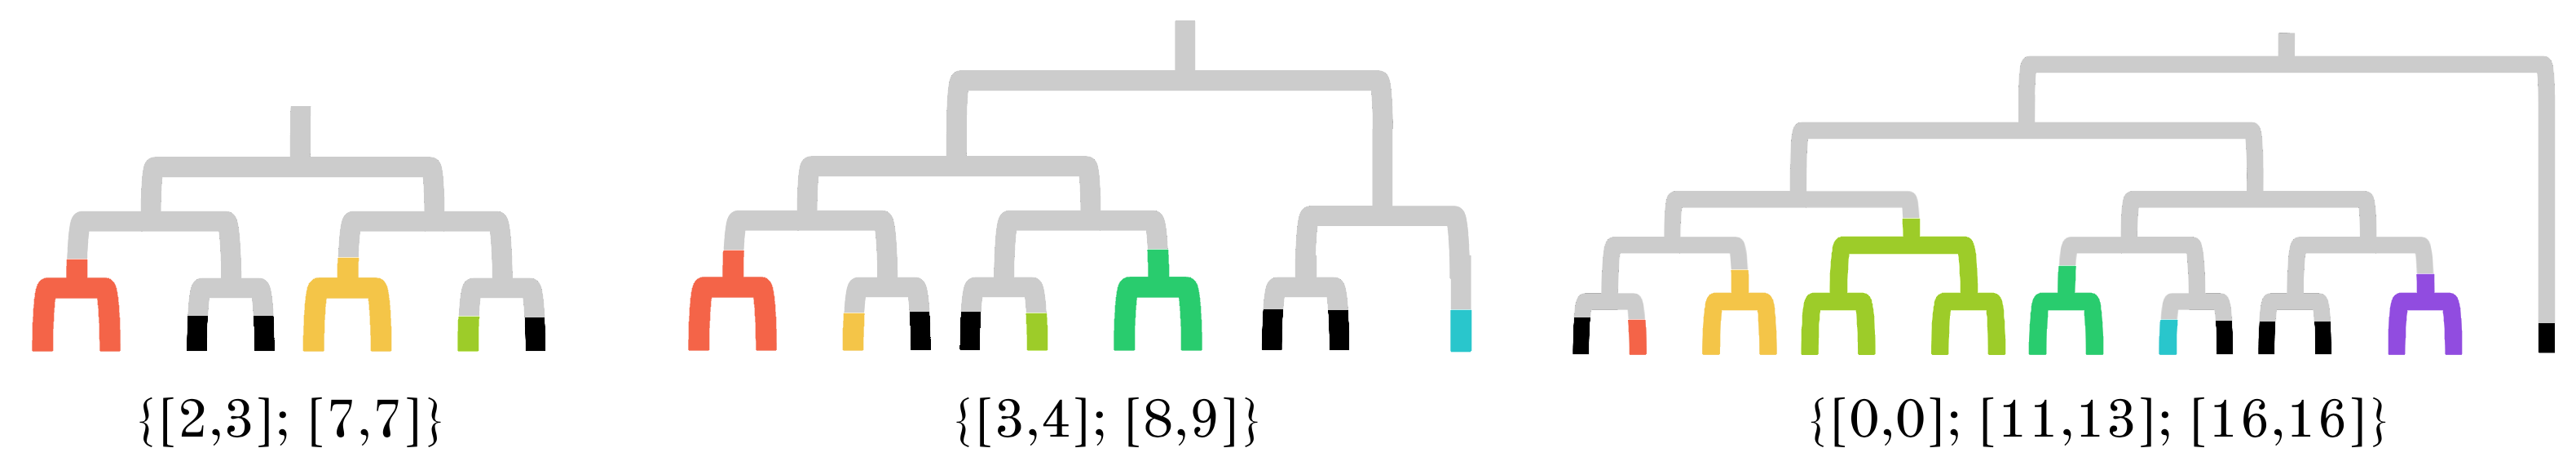
\includegraphics[scale=0.27]{multi}
\centering
\caption{Multi-range Merkle proofs within various BNTs.}
\label{img-multi}
\end{figure*}


\section{Multi-range Proofs}

Generalizing further, we now aim to construct and verify proofs for multiple disjoint ranges within a BNT. Some examples of multi-range proofs are given in Figure \ref{img-multi}.

Encouragingly, the pattern of sibling hashes seems broadly similar to that of the single-leaf and single-range proofs: observe how the subtrees increase in size when moving ``outward'' from each proof range. Knowing this, we're already pretty close to a solution. We can easily confirm, for example, that the sizes of the sibling subtrees to the right of \verb`[0,0]` in Figure \ref{img-multi} match the \verb`0` bits of 0 ($2^0$, $2^1$, $2^2$...), while the sizes of those to the left of \verb`[11,13]` match the \verb`1` bits of 11 ($2^3$, $2^1$, and $2^0$). But how do we know when to stop using the \verb`0` bits of 0, and start using the \verb`1` bits of 11?

For this, we can leverage another property of perfect binary trees: we can compute the ``merge height'' of any two indices by \verb`xor`'ing their bit patterns. This is perhaps more intuitive when the index is interpreted as a path \textit{down} from the root: each bit represents a branch, so as soon as two paths diverge, their bit patterns will begin to differ. \verb`xor` turns matching bits into zeros and differing bits into ones, so to determine when the two paths converge, we simply look for the most significant \verb`1` bit. Thus, the merge height of indices $x$ and $y$ occurs at $\left \lfloor{\log_2(x \oplus y)}\right \rfloor$.

Using the previous example, $000000...\oplus110100... = 110100...$, so these paths merge at height 3. This implies that there cannot be a sibling subtree of size $2^3$ (or larger) between leaves 0 and 11. And this, in turn, tells us to stop using \verb`0` bits of 0 after the 3rd bit, whereupon we switch to using the \verb`1` bits of 11. This produces the sequence $2^0, 2^1, 2^2, 2^1, 2^0$, just as expected.

To encapsulate this operation, we define a new helper procedure, \verb`RangeBits`. For inputs \verb`0` and \verb`11`, \verb`RangeBits` returns \verb`[0,1,2,1,0]`.

\begin{minipage}[c]{0.95\textwidth}
\begin{lstlisting}
fn MergeHeight(x, y):
  return floor(log2(xor(x, y)))
  
fn UpTo(xs, n):
  for i in 0..len(xs):
    if xs[i] > n:
      return xs[0..i]
  return xs
  
fn RangeBits(x, y):
  mh <- MergeHeight(x, y)
  z <- UpTo(zeros(x), mh)
  o <- reverse(UpTo(ones(y), mh))
  return concat(z, o)
\end{lstlisting}
\end{minipage}

\noindent The proof algorithm is then:

\begin{minipage}[c]{0.95\textwidth}
\begin{lstlisting}
fn ProveMultiRange(stream, ranges):
  leaves <- []
  proof <- []
  prev <- not(0)
  for (start, end) in ranges:
    for k in RangeBits(prev, start):
      node <- Subroot(stream, k)
      proof <- append(proof, node)
    for _ in start..end:
      leaf <- readLeaf(stream)
      leaves <- append(leaves, leaf)
    prev <- end
  for k in zeros(prev):
    if empty(stream):
      break
    node <- Subroot(stream, k)
    proof <- append(proof, node)
  return (leaves, proof)
\end{lstlisting}
\end{minipage}

\pagebreak

\noindent As usual, verification is very similar to construction:

\begin{minipage}[c]{0.90\textwidth}
\begin{lstlisting}
fn VerifyMultiRange(ranges, leaves, proof):
  s <- makeStack()
  prev <- not(0)
  for (start, end) in ranges:
    for k in RangeBits(prev, start):
      s <- Insert(s, k, proof[0])
      proof <- proof[1..len(proof)]
    for _ in start..end:
      node <- leafHash(leaves[0])
      leaves <- leaves[1..len(leaves)]
      s <- Insert(s, 0, node)
    prev <- end
  for k in zeros(prev):
    if len(proof) == 0:
      break
    s <- Insert(s, k, proof[0])
    proof <- proof[1..len(proof)]
  return Finalize(s)

\end{lstlisting}
\end{minipage}

We can easily confirm that this algorithm generalizes to the single-range and single-leaf cases. Moreover, it generalizes to \textit{any set of leaves within the tree}, since a range can consist of a single leaf.



\begin{figure*}[t]
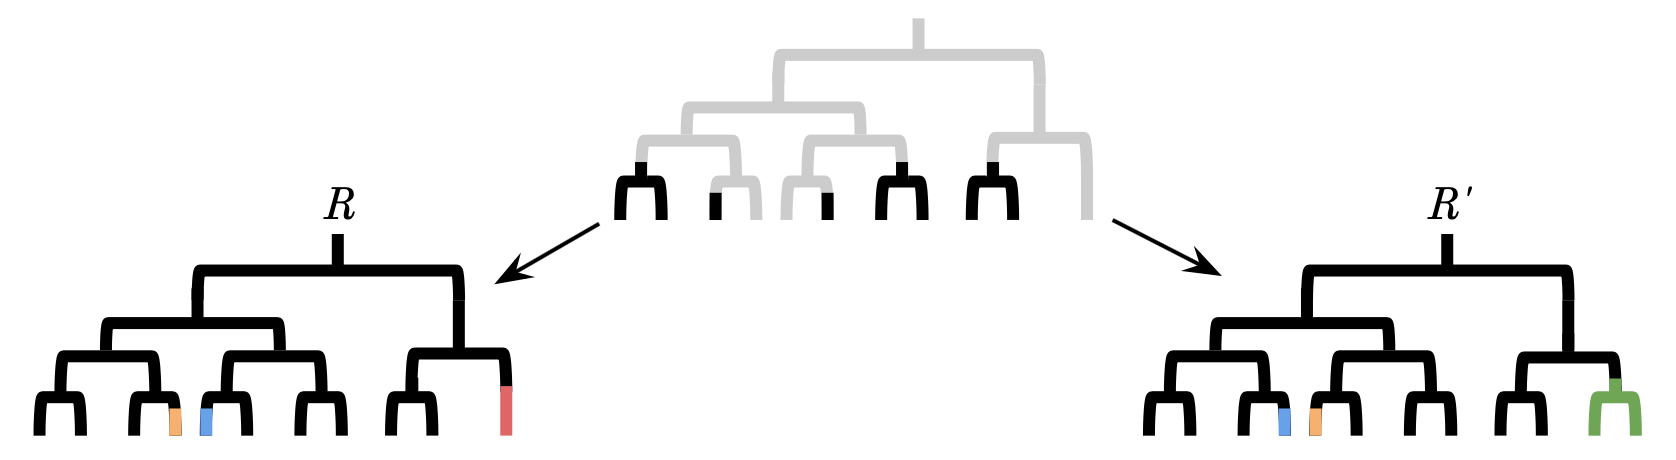
\includegraphics[scale=0.38]{diff}
\centering
\setlength{\belowcaptionskip}{-12pt}
\caption{A Merkle diff proof. Three modifications are applied to the original tree (left): leaf 10 (red) is trimmed; two new leaves (green) are appended; and leaves 3 (orange) and 4 (blue) are swapped, resulting in the new tree (right). The five proof hashes (top), along with the affected leaves, are sufficient to recover the root of either tree.}
\label{img-diff}
\end{figure*}


\section{Diff Proofs}

Building on multi-range proofs, we now introduce a novel type of Merkle proof: the ``Merkle diff proof.'' Diff proofs were created for use in the Sia project, as a solution to the following problem:

Bob is storing multiple terabytes of data on behalf of Alice. The data is represented as a BNT, whose Merkle root $R$ is known to both Alice and Bob. Alice asks Bob to apply some modifications to the data. Bob claims that, after applying the modifications, the new Merkle root is $R'$. How can such a claim be cryptographically verified? In other words, what information can Bob provide to Alice that would allow her to independently compute $R'$?

First, we should define ``modifications'' more precisely. We will restrict ourselves to three operations: appending new leaves to the end of the BNT; trimming leaves from the end of the BNT; and swapping two leaves within the BNT. These operations suffice to achieve any modification. For example, to flip one bit in the middle of the BNT, first append a copy of the leaf with the bit flipped, then swap this leaf with the original, and finally trim the original leaf from the end.

Taken individually, it is not difficult to devise proofs for these operations. To prove an append, Bob supplies the eigenroots of the BNT. Alice can \verb`Insert` these roots into a stack and \verb`Finalize` it, verifying that it produces $R$, then \verb`Insert` the appended leaf and verify that \verb`Finalize` now produces $R'$. The proof for a trim looks much the same, but reversed: Bob provides the post-trim eigenroots (having root $R'$), to which Alice can append the trimmed leaf to produce $R$. Lastly, to prove a swap, Bob provides a multi-range proof for the leaves in the question. Alice can verify that the proof produces $R$, then swap the supplied leaves and recompute the proof to produce $R'$.

For large modifications, though, this approach becomes inefficient. Instead of a separate proof for each operation, we would like to provide and verify a \textit{single} proof for the entire modification; that way, only one pass over the data is required.

We can achieve this by coalescing the set of operations into a set of \textit{affected leaves}---leaves in the original tree that were swapped or trimmed. We then construct a multi-range proof that covers each affected leaf. Such a proof, along with any leaves that Alice is appending, contains all the information that Alice needs to verify the modification. This may become more intuitive when we reframe our problem as follows: \textit{What is the minimal set of leaves and subtree roots that is sufficient to recover both $R$ and $R'$}?

To make things more concrete, we will walk through the proof shown in Figure \ref{img-diff}. Alice requests a modification consisting of three modifications: trimming one leaf, appending two new leaves, and swapping two leaves. In total, three leaves in the old tree are affected (at indices 3, 4, and 10) so Bob computes a multi-range proof for \verb`[[3,4],[10,10]]`, producing the subtree roots shown at the top of the diagram. Bob sends this proof, along with the affected leaves, to Alice. Alice then runs \verb`VerifyMultiRange` on this proof, confirming that it produces $R$. Next, she \textit{applies the modifications locally} to the leaves and ranges: she removes leaf 10, appends the two new leaves, and swaps the positions of leaves 3 and 4. She also removes the \verb`[10,10]` proof range, and adds a new range, \verb`[10,11]`, to cover the new leaves. Finally, Alice runs  \verb`VerifyMultiRange` again, using the same subtree hashes, but modified leaves and proof ranges, and confirms that it produces $R'$.

However, there is one complication that must be dealt with. Consider the diff proof for appending a single leaf: none of the leaves in the original tree were affected, so Bob would compute an empty multi-range proof. But this is incorrect: what we really need is the eigenroots of the original tree. To account for this, we need to make a small tweak to our multi-range algorithms: in the final \verb`for` loop, instead of looping over \verb`zeros(prev)`, we loop over \verb`RangeBits(prev, n)`, where \verb`n` is the size of the tree. This ensures that Bob's proof will always contain the necessary subtree hashes. (Unfortunately, this also means that diff proofs cannot be computed on trees of unknown size.) We will refer to these modified algorithms as \verb`ProveDiff` and \verb`VerifyDiff`.

%TODO: could compute stack for entire tree as we go?

\section{Proof Sizes}

It is often useful to know the exact number of hashes required for a given proof. For the proof constructor, this would allow the array of proof hashes to be allocated once, instead of requiring dynamic reallocation or excessive preallocation. For the proof verifier, this would allow the size of the proof to be verified before performing any hashing.

In a perfect tree with $n$ leaves, a single-leaf proof requires exactly $\log_2(n)$ hashes, since the path from leaf to root includes a sibling hash at each level of the tree. But in a BNT, we must account for the fact that some paths may not have a sibling hash at each level: the left-hand hashes will always be present, but some right-hand hashes may be missing. We can identify these from the path of leaf $n-1$: after the path of leaf $i$ intersects this path, it cannot have any more right-hand hashes. So we adjust our algorithm as follows: we count the number of \verb`1` bits in $i$ to get the number of left-hand hashes; we then compute the merge height of $i$ and $n-1$, and count only the \verb`0` bits up to this height:

\begin{minipage}[c]{0.95\textwidth}
\begin{lstlisting}
fn ProofSize(i, n):
  left <- len(ones(i))
  mh <- MergeHeight(i, n-1)
  right <- len(UpTo(zeros(i), mh))
  return left + right
\end{lstlisting}
\end{minipage}

As it so happens, the same approach works for single-range proofs: we just need to count the \verb`0` bits of the end index instead of the start index. As a degenerate case, a proof size of 0 occurs when the range covers the entire tree; conversely, the largest proof size, $2\log_2(n)$, occurs when the range covers the two leaves in the middle of a perfect tree.

Multi-range proofs are more complicated, but we can reuse our existing proof algorithm:

\begin{minipage}[c]{0.95\textwidth}
\begin{lstlisting}
fn ProofSizeMulti(ranges, n):
  s <- 0
  prev <- not(0)
  for (start, end) in ranges:
    s <- s + ProofSize(prev, start)
    prev <- end
  mh <- MergeHeight(prev, n-1)
  s <- s + len(UpTo(zeros(prev), mh))
  return s
\end{lstlisting}
\end{minipage}

For a set of $k$ ranges evenly distributed throughout the tree, the proof requires $k\left \lfloor{\log_2(n/k)}\right \rfloor$ hashes. The largest possible proof therefore results from a set of $n/2$ ranges, covering every other leaf; this requires $n/2$ hashes.

Lastly, since diff proofs are just multi-range proofs with possible trailing eigenroots, we can implement \verb`ProofSizeDiff` by modifying \verb`ProofSizeMulti` to include the final \verb`ones` as well as the \verb`zeros`. This actually simplifies the algorithm, because we can reuse \verb`ProofSize`:

\begin{minipage}[c]{0.1\textwidth}
\begin{lstlisting}
fn ProofSizeDiff(ranges, n):
  s <- 0
  prev <- not(0)
  for (start, end) in ranges:
    s <- s + ProofSize(prev, start)
    prev <- end
  s <- s + ProofSize(prev, n)
  return s
\end{lstlisting}
\end{minipage}


\section{Hardware Sympathy}

% TODO move description of stack here?

In the algorithms presented above, we assume the existence of functions like \verb`ones` and \verb`log2` for simplicity. In practice, we can replace these functions with far more efficient methods. In particular, instead of allocating and populating arrays of bit positions, our loops should iterate directly over the bits themselves, using shifts and masking operations to select \verb`1` or \verb`0` bits as necessary. Furthermore, virtually all processors support a native instruction for obtaining the position of the most significant \verb`1` bit (e.g. \verb`bsr` on x86), which is equivalent to $\left \lfloor{\log_2(x)}\right \rfloor$. Thus our \verb`MergeHeight` function can be implemented in as little as two instructions.

We can optimize our proof size algorithms even more aggressively by using the \verb`popcnt` instruction, which returns the number of \verb`1` bits in an integer. To implement \verb`ProofSize`, we can use one \verb`popcnt` to obtain the number of \verb`1` bits, and another---after taking the complement and applying a mask---to obtain the number of \verb`0` bits. In total, \verb`ProofSize` only requires about a dozen instructions.  % TODO appendix? link to godbolt?

But far greater performance improvements can be achieved through the use of SIMD instructions, which (among other things) allow us to compute multiple hash digests simultaneously. This capability can be directly applied to computing Merkle roots. Instead of hashing each leaf immediately after reading it from the stream, an implementation can buffer $p$ leaves in memory, then hash all of them together. The resulting digests can then be hashed together to produce a single root, which is inserted into the stack.

Another approach is to redefine the stack itself. Instead of storing one root per depth, a $p$-stack can store $p$ roots per depth. When the next $p$ leaves are hashed, the digests can be inserted into this stack directly. Of course, the same merging rules apply: if the ``slot'' for that depth is already occupied, the two groups are hashed together to form a new set of digests, and the insertion process recurses at a higher depth. This approach allows us to use SIMD routines for hashing both leaves and roots.

%To minimize copying, the stack should be stored in ``big-endian'' order. This makes it possible to combine adjacent stack elements directly, at the cost of making stack manipulations more complex.

% TODO: real-world performance data/graphs?

\section{Conclusion}

We introduced the binary numeral tree and explored how its structure lends itself to elegant and efficient algorithms on streams of arbitrary size. We then presented algorithms for constructing single-leaf, single-range, multi-range, and ``diff'' Merkle proofs within BNTs, and complementary algorithms for computing the size of each such proof. Each algorithm requires a single pass over the data and $\mathcal{O}(\log_2(n))$ space. Finally, we discussed how specialized CPU instructions can be leveraged to greatly improve the performance of these algorithms.

\section{Acknowledgements}

Thanks to David Vorick and Ben Jones for many fruitful discussions of Merkle trees. Thanks to Jack O'Connor and Samuel Neves for inspiration and advice on SIMD hashing. Thanks to Lum Ramabaja for inspiring me to publish these results.

\bibliographystyle{plain}
\bibliography{references.bib}

% appendix: asm https://godbolt.org/z/xPrMPx

\end{document}
